\documentclass[10pt]{article}
\usepackage{main,times}

\input{math_commands.tex}

\usepackage[UTF8,scheme=plain,zihao=false]{ctex}
\setCJKmainfont{Songti SC}
\setCJKsansfont{PingFang SC}
\setCJKmonofont{Songti SC}
\usepackage[colorlinks=true,linkcolor=blue,citecolor=blue,urlcolor=blue]{hyperref}
\usepackage{url}
\usepackage{booktabs}
\usepackage{amsfonts}
\usepackage{nicefrac}
\usepackage{microtype}
\usepackage{xcolor}
\usepackage{graphicx}
\usepackage{float}
\usepackage{caption}
\usepackage{enumitem}
\usepackage{array}

\captionsetup{font=small,labelfont=bf}
\renewcommand{\abstractname}{摘要}
\renewcommand{\figurename}{图}
\renewcommand{\tablename}{表}
\renewcommand{\refname}{参考文献}
\renewenvironment{abstract}{%
  \vskip 0.075in
  \centerline{\large\bfseries 摘要}
  \vspace{0.5ex}
  \begin{quote}
}{%
  \par\end{quote}\vskip 1ex
}
\setlength{\parskip}{0.2em}
\setlist{nosep,leftmargin=2em}

\makeatletter
\renewcommand{\chapterautorefname}{\S\@gobble}
\renewcommand{\sectionautorefname}{\S\@gobble}
\renewcommand{\subsectionautorefname}{\S\@gobble}
\renewcommand{\subsubsectionautorefname}{\S\@gobble}
\renewcommand{\appendixautorefname}{\S\@gobble}
\renewcommand{\cite}{\citep}
\makeatother

\title{面向计算机使用的高效智能体训练\\
\large Efficient Agent Training for Computer Use}

\author{Yanheng He\textsuperscript{1,3}\thanks{共同第一作者。~$^\dagger$通讯作者。}\quad
Jiahe Jin\textsuperscript{1,3}$^*$\quad
Pengfei Liu\textsuperscript{1,2,3}$^\dagger$
\\
\textsuperscript{1}上海交通大学\quad
\textsuperscript{2}SII\quad
\textsuperscript{3}GAIR}

\iclrfinalcopy
\begin{document}

\maketitle

\begin{abstract}
长期以来，扩充高质量轨迹数据一直是开发类人计算机使用智能体的关键瓶颈。我们提出 PC Agent-E，这是一种高效的智能体训练框架，可显著降低对大规模人类演示的依赖。我们仅从 \textbf{312} 条人工标注的计算机使用轨迹出发，再利用 Claude 3.7 Sonnet 合成多样化的替代动作决策，从而对这些轨迹进行增强。在这些扩充后的轨迹上训练得到的 PC Agent-E 模型取得了显著的 \textbf{141\%} 相对提升；在我们同时发布的改进基准 WindowsAgentArena-V2 上，其表现甚至相对超过 Claude 3.7 Sonnet \textbf{10\%}。通过将可靠的人类计算机使用技能与自动化 AI 数据合成能力相结合，我们的方法不仅相较于仅在人类轨迹上训练带来了大幅提升，也显著优于对 Claude 3.7 Sonnet 的直接蒸馏。代码、数据和模型见 \url{https://github.com/GAIR-NLP/PC-Agent-E}。
\end{abstract}

\section{引言}
\label{sec: intro}

\begin{figure}[H]
  \centering
  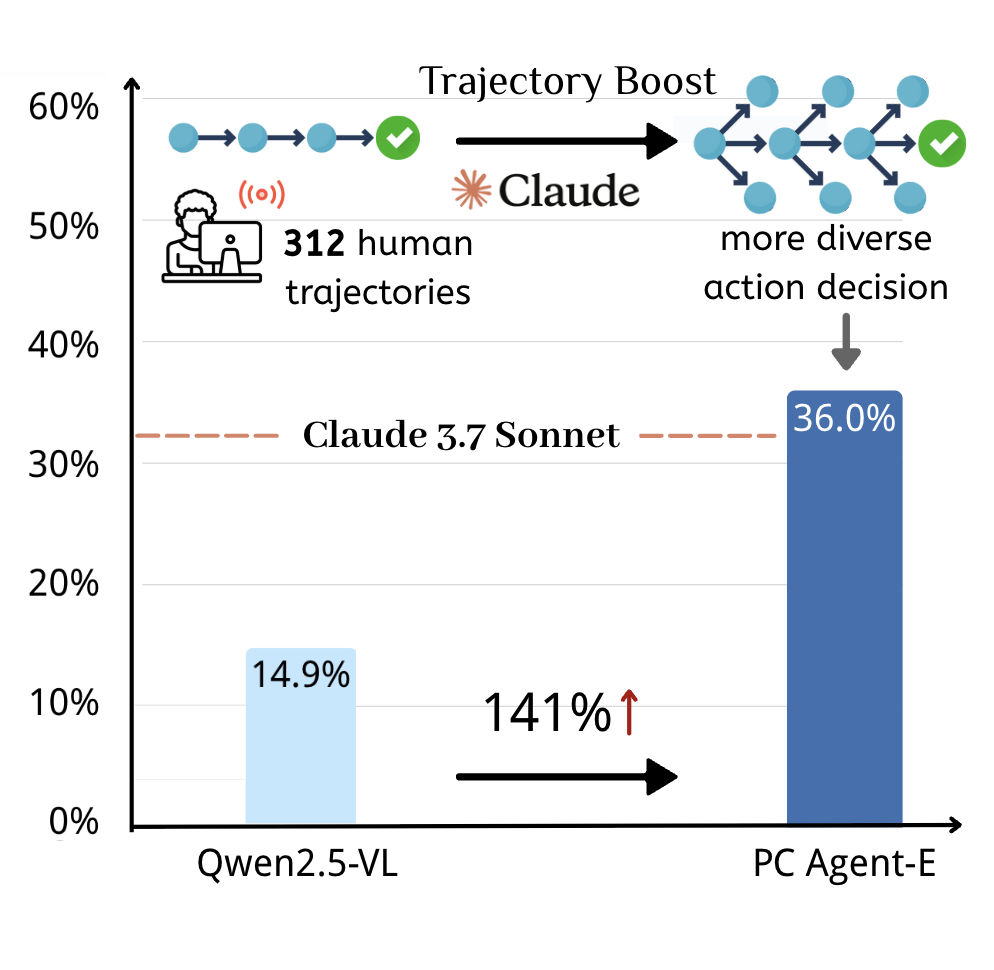
\includegraphics[width=0.45\linewidth]{assets/first_image.png}
  \caption{PC Agent-E 仅使用 312 条增强轨迹，便在 Windows 计算机使用任务上取得了开源模型中的最佳性能。}
  \label{fig:first_image}
\end{figure}

开发能够像人类一样操作计算机的自主智能体~\cite{2024claudecomputeruse,2025openaicua}，长期以来一直是人工智能领域的标志性追求。此类计算机使用智能体由视觉语言模型（VLM）驱动，通过感知屏幕截图直接与图形用户界面（GUI）交互，例如点击按钮、浏览菜单和输入文本。这使其能够自动化广泛的数字任务，从日常文书工作和网上购物到复杂的内容创作都有覆盖，并有望显著减少人类的手工工作量。

然而，现有模型的表现仍显著落后于人类~\cite{xie2024osworldbenchmarkingmultimodalagents,bonatti2024windowsagentarenaevaluating}。这一能力差距在开源社区中更为明显：目前尚无开源方案能够与 Claude 3.7 Sonnet 等领先的专有系统竞争~\cite{2025claude37}。如何让开源模型掌握这些高级计算机使用能力，仍是一个尚未解决的问题。造成这一不足的关键因素之一，是高质量计算机使用轨迹数据极度稀缺~\cite{ou2024synatraturningindirectknowledge,xu2025agenttrekagenttrajectorysynthesis}。

本文研究面向计算机使用的高效智能体训练，目标是在只需极少人工标注的情况下，使开源模型的表现甚至超过专有模型。近期研究~\cite{huang2024o1,muennighoff2025s1,ye2025limo}发现，使用 Deepseek-R1~\cite{guo2025deepseek} 等先进推理模型合成高质量数据，可以高效增强大语言模型的推理能力；受此启发，我们将类似思路扩展到计算机使用智能体领域。

我们提出 \textbf{PC Agent-E}，一种融合人类专长与 AI 自动化的高效智能体训练框架。该框架从一小组真实世界的人类计算机使用轨迹出发，借助前沿智能体模型使动作决策多样化，从而产生更丰富的监督信号。在这些增强轨迹上训练后，我们的智能体以突出的数据效率展现出强大的计算机使用能力。

首先，我们使用收集人机交互数据的 PC Tracker~\cite{he2024pcagentsleepai}，由两名人员在一天内标注并收集了 \textbf{312} 条人类计算机使用轨迹。这些轨迹包含任务描述、屏幕截图，以及人类的键盘和鼠标动作。随后，我们重建人类动作背后的隐式思考过程，得到包含思考内容的完整人类轨迹。由于人类能够熟练完成这些任务，其成功完成本身已有保证，因此不需要额外验证。

这些人类轨迹已经是有价值的智能体训练数据；在此基础上，我们又通过自行设计的数据合成方法 \textbf{Trajectory Boost} 对其进行增强，为轨迹的每一步补充多样化的替代动作决策。其核心洞见是：计算机使用任务往往可以通过多条有效路径完成，因此在每一步，都可能存在若干由合理思考支持的可行动作选项。为了捕捉这种多样性，我们使用强智能体模型合成其他可能的动作决策。具体而言，人类轨迹中的每一步都提供了一个 \textbf{\textit{环境快照}}，其中包含计算机使用智能体作出决策所必需的关键状态信息。我们将这些快照提供给 Claude 3.7 Sonnet，并采样多个可能的动作决策，从而显著扩充轨迹数据并提高其多样性。

实验结果表明，只需一小组人工标注轨迹，我们的方法就能将开源模型的性能提升至前沿模型的水平。PC Agent-E 仅使用由 Claude 3.7 Sonnet 增强的 312 条轨迹进行训练，便在 \textbf{WindowsAgentArena-V2} 上相较基础模型 Qwen2.5-VL-72B 取得了令人瞩目的 \textbf{141\%} 相对提升，甚至相对超过教师模型 Claude 3.7 Sonnet 10\%。WindowsAgentArena-V2 是我们在 WindowsAgentArena~\cite{bonatti2024windowsagentarenaevaluating} 基础上改进的基准。此外，PC Agent-E 在 OSWorld~\cite{xie2024osworldbenchmarkingmultimodalagents} 上也能良好泛化至不同操作系统。消融实验进一步表明，我们利用人类演示的方法不仅优于仅依赖原始人类轨迹，也比直接蒸馏教师模型显著更有效、更高效。

\begin{figure}[t]
    \centering
    
\includegraphics[width=\linewidth]{assets/overview.png}
    \caption{本文框架概览，包含四个关键组成部分：（1）轨迹收集：记录用户每一步的动作和状态观测，获得一小组人类轨迹；（2）思考补全：重建原始人类轨迹中缺失的隐式思考过程；（3）Trajectory Boost：使动作决策多样化，从而进一步增强轨迹；（4）智能体训练：以出色的数据效率训练强大的计算机使用智能体。}
    \label{fig: method overview}
\end{figure}

总之，本文的主要贡献有三点：

\begin{enumerate}
    \item 我们提出 \textbf{Trajectory Boost}，这是一种简单的数据合成方法，可为计算机使用智能体训练释放显著的数据效率。该方法以一个前沿模型生成的多样化动作决策增强人类轨迹；与仅使用人类数据和直接蒸馏相比，它都表现出显著更高的有效性和效率。
    \item 我们发布 \textbf{WindowsAgentArena-V2}。这一改进基准修复了原始 WindowsAgentArena 中的评估依赖、不可行任务投机以及其他局限，从而对计算机使用能力作出更稳健、更公平的评估。
    \item 我们开发了 \textbf{PC Agent-E}，这是一个性能可媲美领先专有模型的开源计算机使用智能体。该模型仅使用 312 条增强轨迹进行训练，便成功超过强教师模型 Claude 3.7 Sonnet，展现出卓越的数据效率。
\end{enumerate}

\section{相关工作}
\label{gen_inst}

\subsection{计算机使用智能体}

随着 VLM 不断发展~\cite{bai2025qwen25vltechnicalreport,deitke2024molmo}，计算机使用智能体与计算机交互的方式逐渐从依赖无障碍树等文本表示~\cite{2024agents,wu2024oscopilot}，转向直接使用屏幕截图~\cite{uitars2025,xu2025aguvisunifiedpurevision,he2024pcagentsleepai}。根据设计中引入人类先验的程度，现有计算机使用智能体可分为两类：一类是\textit{模块化智能体工作流}~\cite{2024agents,wu2024oscopilot}，其定义专用模块，并通过提示让多个智能体协作；另一类是\textit{原生智能体模型}~\cite{2024claudecomputeruse,uitars2025,2025openaicua}，其依赖单一模型根据历史和当前状态逐步采取动作。

模块化智能体工作流虽然可以降低任务复杂度，但其对人类先验的高度依赖会妨碍对新领域的适应，并限制端到端优化~\cite{SaltzerReedClark1984end2end,pan2024swegym}。随着模型能力持续增强，原生智能体模型已经成为主导范式。该方法具有灵活性和泛化能力，并能通过监督微调（SFT）~\cite{xu2025aguvisunifiedpurevision}或强化学习（RL）~\cite{2025openaicua}获得可持续的性能增益。本文通过 SFT 探索原生智能体模型的高效训练方法。

\subsection{数据合成}

随着大语言模型（LLM）的能力日益增强，使用它们合成数据已成为常见做法。蒸馏方法~\cite{taori2023alpaca,gunasekar2023textbooksneed,xu2023wizardlmempoweringlargelanguage}利用最先进的（SOTA）模型生成大规模数据，以训练能力较弱的模型；另一方面，自我改进方法使模型能够自行引导并优化其训练数据~\cite{wang2023selfinstructaligninglanguagemodels2}。

在计算机使用智能体领域，数据合成大致可分为三类：（1）构建 GUI 基础理解的大规模数据集，其中包括屏幕截图描述或问答等任务~\cite{liu2024harnessingwebpageuistextrich,uitars2025}；（2）单步视觉定位，即从 GUI 上的特定位置合成鼠标点击任务~\cite{gou2025navigatingdigitalworldhumans,wu2024osatlasfoundationactionmodel}；（3）多步轨迹，近期研究或利用网页教程引导轨迹生成~\cite{ou2024synatraturningindirectknowledge,xu2025agenttrekagenttrajectorysynthesis}，或根据智能体自身的探索记录反向合成任务~\cite{sun2025osgenesisautomatingguiagent,murty2024nnetscape}。与以往工作不同，本文基于真实世界的人类演示合成高质量多步轨迹，并强调数据效率。

\section{方法}

\subsection{概览}

如图~\ref{fig: method overview} 所示，我们提出 PC Agent-E，这是一种面向计算机使用的高效智能体训练框架，将人类专长与 AI 自动化相结合。我们的方法将真实的人机交互与多样化的动作决策结合起来，生成高质量轨迹数据，兼具真实性与多样性。

\begin{enumerate}
    \item 首先，我们从人类标注者处收集一小组 312 条任务轨迹，记录每一步的屏幕状态观测和人类动作，随后过滤数据，移除错误的步骤和轨迹。（\autoref{sec: traj collection}）
    \item 然后，我们根据对应的屏幕状态观测和历史步骤上下文，重建每次动作决策之前人类潜在的思考过程。（\autoref{sec: thought completion}）
    \item 接下来，我们将人类轨迹作为\textit{环境快照}，使用 Claude 3.7 Sonnet 和 Trajectory Boost 方法合成多样化的替代动作决策。（\autoref{sec:trajboost}）
    \item 最后，我们在增强轨迹上以简单的端到端支架训练 PC Agent-E，使其成为面向 Windows 计算机使用的 SOTA 原生智能体模型。（\autoref{sec: agent training}）
\end{enumerate}

\subsection{轨迹收集}
\label{sec: traj collection}

\begin{figure}[t]
  \centering
  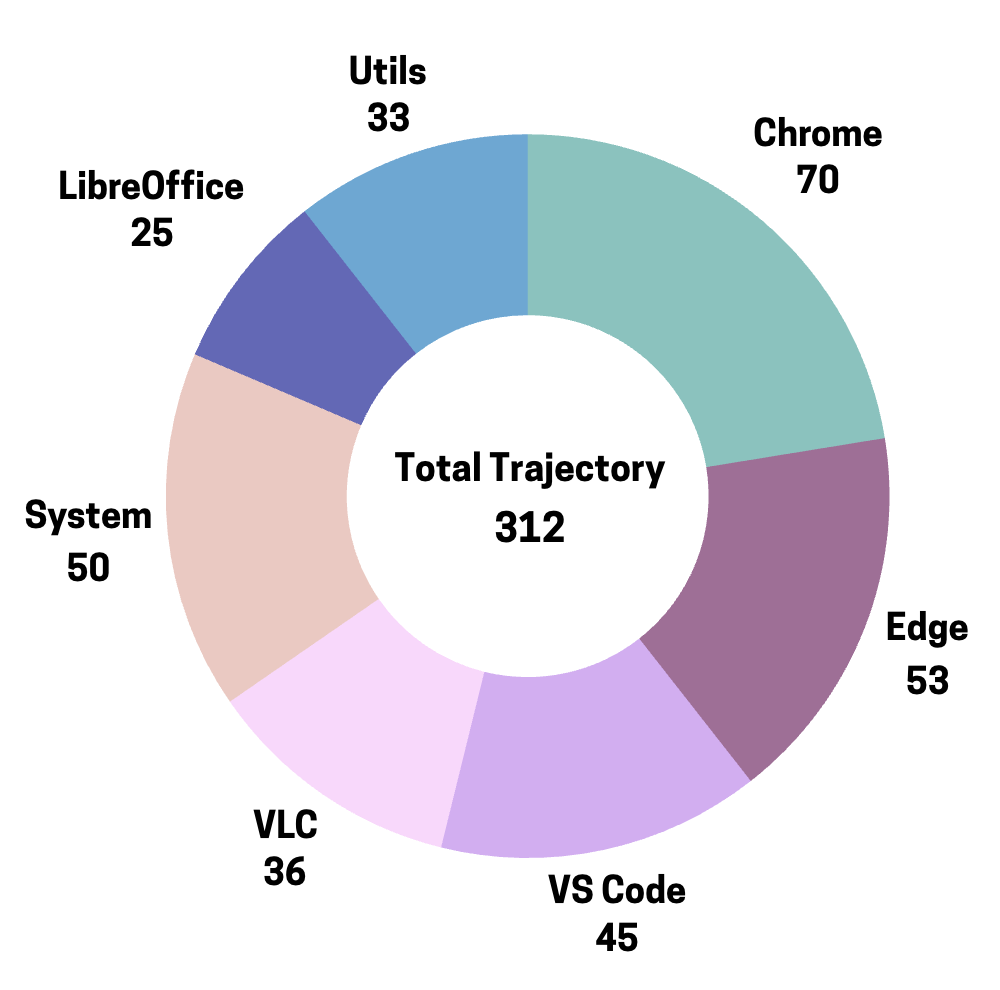
\includegraphics[width=0.42\linewidth]{assets/data_distribution.png}
  \caption{312 条任务轨迹在不同应用程序中的分布。}
  \label{fig:data distribution}
\end{figure}

\begin{table}[t]
  \centering
  \small
  \begin{tabular}{lcc}
  \toprule
  \textbf{长度范围} & \textbf{数量} & \textbf{比例} \\
  \midrule
  2--5   & 74  & 23.7\% \\
  6--10  & 139 & 44.6\% \\
  11--15 & 73  & 23.4\% \\
  16--30 & 26  & 8.3\%  \\
  \bottomrule
  \end{tabular}
  \caption{312 条任务轨迹在不同长度范围（步数）上的分布。}
  \label{tab:traj_length_dist}
\end{table}

我们使用 PC Tracker~\cite{he2024pcagentsleepai} 收集人类计算机使用轨迹。对于给定任务，该工具会记录每一步的屏幕状态观测和人类键盘或鼠标动作。记录的动作被结构化为表~\ref{tab:action-space} 所示的统一动作空间 $\mathcal{A}$。在生成任务时，我们首先跨多个软件应用人工编写一小组种子任务，再使用 LLM 扩展任务集合。随后将所得任务分配给人类标注者；标注者在自己的 Windows 计算机上完成任务，同时由 PC Tracker 自动记录轨迹。完成任务后，标注者可以丢弃不满意的轨迹，也可根据实际执行修改任务描述，从而保证所收集轨迹的正确性和完整性。之后，我们采用一组基于规则的过滤器，移除存在错误或其他不良行为的整条轨迹或单个步骤。

我们对所收集的轨迹执行了严格的数据去污染流程。使用 n-gram 重叠度和语义相似度指标，将每条任务描述与主评估基准（\autoref{sec:waa-v2}）中的任务进行比较。具体而言，只有当一条轨迹的任务描述与任一测试任务之间的 13-gram 重叠为 0、3-gram 重叠低于 0.7，且余弦语义相似度低于 0.85 时，我们才保留该轨迹。

该流程最终得到 312 条真实世界的人类计算机使用轨迹，其应用程序分布见图~\ref{fig:data distribution}，轨迹长度分布见表~\ref{tab:traj_length_dist}。我们没有向标注者明确规定轨迹长度；这一分布自然产生于所收集的任务和人类演示行为。整个标注过程由两名标注者在一天内完成，平均每条轨迹约需 3 分钟。考虑到人类对计算机使用十分熟练、标注者可以在执行后丢弃轨迹或修改任务描述，且我们还执行了数据过滤，因此无须额外验证轨迹的正确性。

\begin{table}[t]
\centering
\small
\resizebox{0.9\linewidth}{!}{%
\begin{tabular}{@{}lp{7.3cm}@{}}
\toprule
\textbf{动作} & \textbf{说明} \\ \midrule
\textit{click (x, y)} & 在指定坐标单击。 \\
\textit{right click (x, y)} & 在指定坐标右键单击。 \\
\textit{double click (x, y)} & 在指定坐标双击。 \\
\textit{drag from (x1, y1) to (x2, y2)} & 拖动鼠标。 \\
\textit{scroll (x)} & 以偏移量 x 滚动屏幕。 \\
\textit{press key: enter} & 按下 Enter 键。 \\
\textit{hotkey (ctrl, c)} & 执行 Ctrl+C 快捷键。 \\
\textit{type text: hello} & 输入文本 ``hello''。 \\
\textit{wait} & 暂停一段时间。 \\
\textit{finish} & 任务已完成。 \\
\textit{fail} & 任务失败。 \\ \bottomrule
\end{tabular}%
}
\caption{统一动作空间 $\mathcal{A}$。}
\label{tab:action-space}
\end{table}

\subsection{思考补全}
\label{sec: thought completion}

我们首先以迭代方式重建人类动作背后的隐式思考过程。具体而言，对于原始轨迹中的每个动作，我们向 Claude 3.7 Sonnet 提供任务描述、历史动作及此前已重建的思考过程、当前动作和对应的屏幕截图。模型根据这些信息生成该动作背后的隐式思考过程。如图~\ref{fig:trajboost} 所示，记录得到的原始人类轨迹会被转换为包含思考内容的人类轨迹，即在每一步中加入重建的思考过程。所用提示见原文附录 F.1。

\subsection{Trajectory Boost}
\label{sec:trajboost}

完成思考补全后，我们获得了包含显式思考过程的完整人类轨迹。尽管这些轨迹已经是有价值的智能体训练样本，我们仍使用一种简单但有效的方法 \textbf{Trajectory Boost} 进一步增强它们，为轨迹中的每一步合成多样化的替代动作决策。

Trajectory Boost 的动机在于，计算机使用任务天然允许多条有效的求解路径。因此，在任意给定步骤，除了人类标注者采用的单一方案，还可能存在若干由合理思考过程支持的可行动作。为了捕捉这种内在多样性，我们使用前沿计算机使用智能体 Claude 3.7 Sonnet 生成单步替代动作决策。它的长程规划能力、先进推理模式和广泛的计算机使用知识，使其能够生成信息量大且有价值的思考过程与动作，从而大幅提升轨迹数据的丰富度和多样性。

具体而言，我们注意到，人类轨迹的每一步都记录了计算机的一个\textit{环境快照}，提供人类和智能体作出决策所需的信息。对于一条人类轨迹中的第 $k$ 步，设观测为 $o_k$、思考过程为 $t_k$、动作为 $a_k$、任务描述为 $T$，则\textit{环境快照}为 $<T,o_k,h_k>$，其中历史上下文 $h_k=(t_1,a_1,t_2,a_2,\dots,t_{k-1},a_{t-1})$ 由此前的人类步骤构成。我们将该\textit{环境快照}输入实例化于 PC Agent-E 支架（\autoref{sec: agent training}）中的 Claude 3.7 Sonnet，并从中采样多个单步动作决策 $(t_k',a_k')$。所用提示见原文附录 F.2。在实践中，我们并行采样 9 个动作决策。由此得到图~\ref{fig:trajboost} 所示的 \textbf{\textit{Traj Tree}}：人类轨迹构成主干，增强后的动作决策作为叶节点分叉出去。这些由 Claude 3.7 Sonnet 采样的动作决策不会在真实计算机环境中执行，但会作为后续智能体训练的重要增强数据。

\begin{figure}[t]
    \centering
    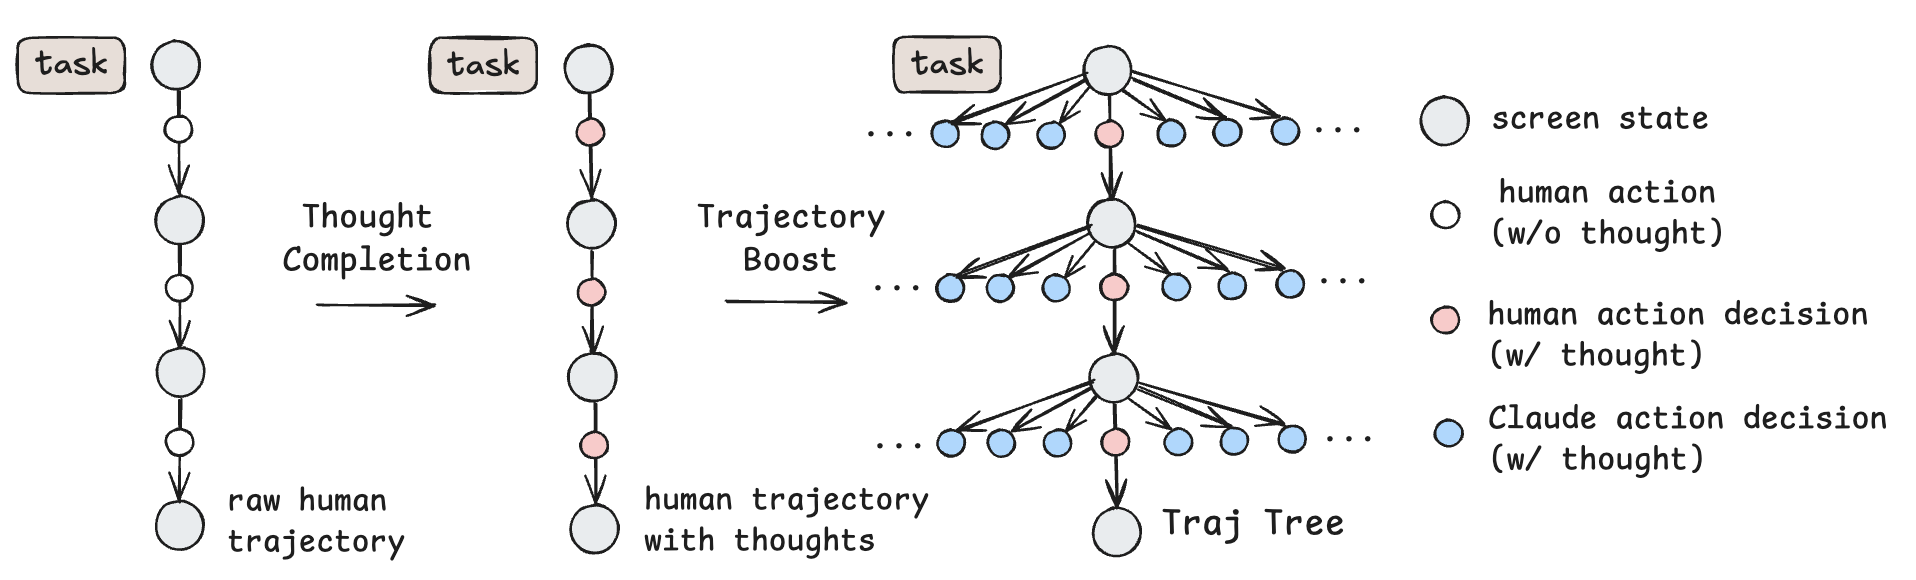
\includegraphics[width=\linewidth]{assets/trajboost.png}
    \caption{Trajectory Boost 方法示意图。（左）PC Tracker 记录的原始人类轨迹。（中）经过思考补全、加入重建思考过程后的人类轨迹，其中红色节点表示人类动作决策。（右）最终的 \textit{Traj Tree}，其中蓝色节点表示 Claude 3.7 Sonnet 合成的多样化增强动作决策。}
    \label{fig:trajboost}
\end{figure}

\subsection{智能体训练}
\label{sec: agent training}

\begin{figure}[t]
    \centering
    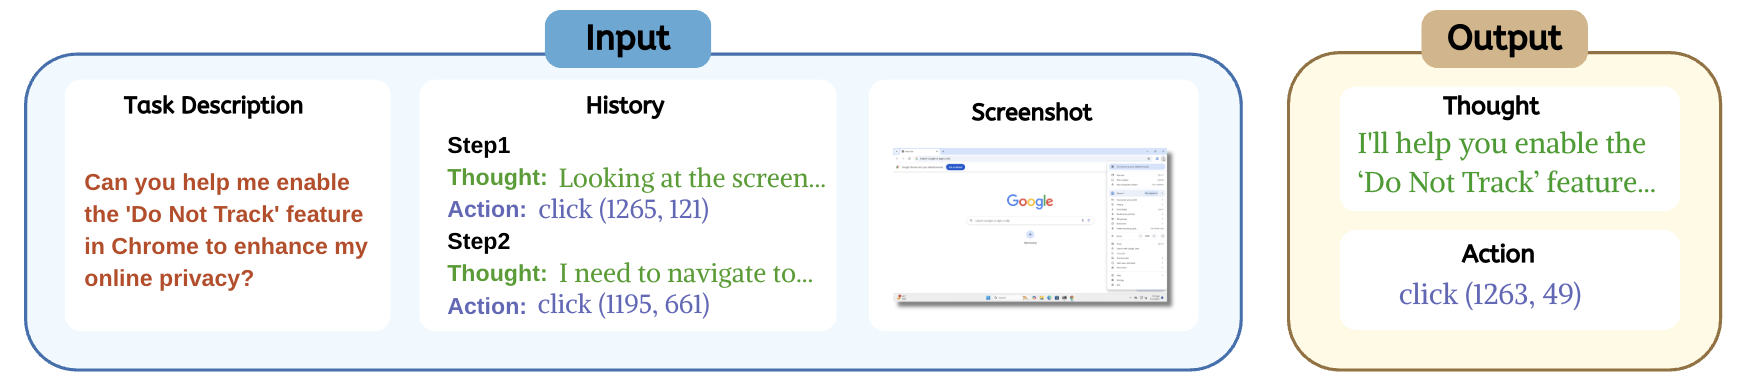
\includegraphics[width=\linewidth]{assets/scaffold.png}
    \caption{一个训练样本，同时展示 PC Agent-E 支架的推理过程。}
    \label{fig:scaffold}
\end{figure}

PC Agent-E 有意采用简单的端到端支架，因为我们的首要目标是验证智能体训练方法的有效性，而非通过复杂的工作流设计或精巧的提示工程优化性能。在推理时，如图~\ref{fig:scaffold} 所示，PC Agent-E 以 $\langle$屏幕截图、任务描述、历史$\rangle$ 为输入，按照 ReAct~\cite{yao2023reactsynergizingreasoningacting} 范式输出 $\langle$思考、动作$\rangle$ 决策。动作空间与表~\ref{tab:action-space} 中的 $\mathcal{A}$ 相同，每个动作均通过 \texttt{PyAutoGUI} 库执行。历史是此前思考与动作的文本日志。为在训练和推理中保持简洁，我们不包含过去的屏幕截图；不过，作者认为加入这些图像历史有助于提高模型性能。支架所用提示见原文附录 F.3。

在训练时，我们将 \textit{Traj Tree} 中的每个动作节点转换为一个独立训练样本。如图~\ref{fig:scaffold} 所示，训练样本的结构与智能体在推理时采用的支架直接对应。对于人类演示和模型合成的动作节点，训练样本中的历史都只包含 \textit{Traj Tree} 主干上先前的人类动作。这与人类或模型作出相应动作决策时可获得的历史上下文一致。最终，我们从 312 条增强轨迹中获得了 27K 个训练样本，每个样本都遵循与推理时一致的输入输出结构。

\section{WindowsAgentArena-V2}
\label{sec:waa-v2}

\begin{figure}[t]
    \centering
    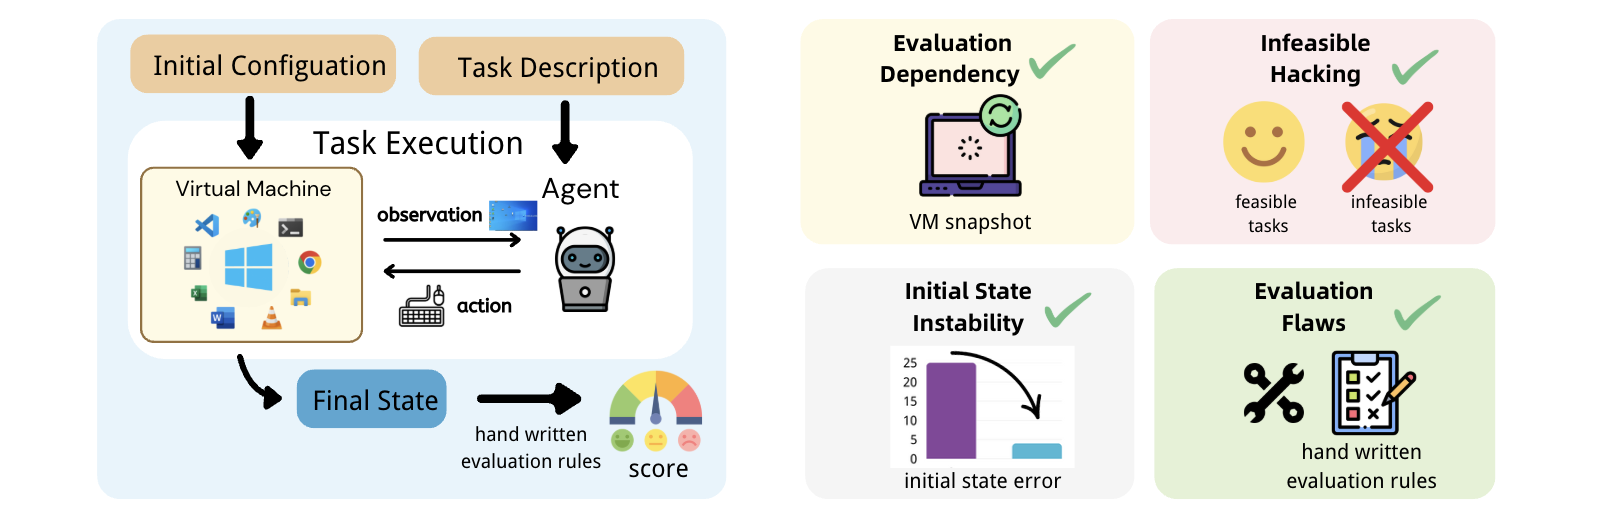
\includegraphics[width=\linewidth]{assets/waa.png}
    \caption{（左）WindowsAgentArena 基准概览。（右）我们对更新后的 WindowsAgentArena-V2 基准所作的主要修改。}
    \label{fig:waa-v2}
\end{figure}

我们最初在 WindowsAgentArena~\cite{bonatti2024windowsagentarenaevaluating} 上进行评估。该基准旨在通过跨多个应用程序的多样化任务，在真实的 Windows 操作系统环境中评估计算机使用能力。它可以自动配置虚拟机（VM）的初始状态，并提供人工编写的评估规则（见图~\ref{fig:waa-v2}）。不过，我们在评估过程中发现了若干局限。为了保证评估可靠性，我们开发了 \textbf{WindowsAgentArena-V2}。这一更新后的基准包含来自 11 个常用 Windows 应用程序的 141 个任务，全部源自原始 WindowsAgentArena，并作出如下改进。

\paragraph{解决评估依赖问题。}
原始基准没有在任务评估之间重置 VM 状态，因此先前任务造成的变化可能影响后续任务。我们在每次评估前恢复 VM 快照，以保证起始状态一致，防止任务之间相互干扰，并满足 i.i.d.（独立同分布）假设。我们还安装了原始 VM 快照中缺失、但正确评估所必需的一些软件。

\paragraph{防止对不可行任务投机。}
WindowsAgentArena 和 OSWorld 等现有计算机使用基准通常包含不可行任务；由于系统功能已被弃用或用户生成的命令存在臆造等原因，这些任务本质上无法完成~\cite{xie2024osworldbenchmarkingmultimodalagents}。此类任务的评估指标非常简单：只要智能体在执行过程中的任意时刻输出动作 \texttt{FAIL}，便将任务视为成功。然而，我们发现这种评估方法特别容易被投机利用：智能体只需始终输出 \texttt{FAIL}，便可在不可行任务上轻易取得满分，而无须展示任何有意义的计算机使用能力。相比之下，完成可行任务通常要求智能体逐步执行动作，真正实现任务目标，难度层级显著不同。

我们将这一现象称为 \textbf{\textit{不可行任务投机}}。后续实验（\autoref{subsec: osworld}）验证了这一漏洞：一个较弱的模型在不可行任务上反而取得显著更高的分数。由于可行任务与不可行任务的得分相同，二者并存会损害基准公平性。此外，鉴于当前计算机使用智能体的能力距离理想水平仍很远，作者认为现阶段更有价值的是着重提升智能体在可行任务上的表现。因此，作为 WindowsAgentArena-V2 中的一项临时解决方案，我们移除了所有不可行任务，以防止\textit{不可行任务投机}。

\paragraph{保证 VM 初始状态稳定。}
我们发现，任务初始配置完成后的 VM 状态经常出现网络连接不稳定、软件启动失败或系统卡顿等错误。为此，我们设计了一个结合基于规则评估和基于 LLM 评估的验证框架，用于检查初始状态；对于有问题的初始化，还提供最多三次重启尝试的重测机制。该方法将初始化失败率从 10\%--30\%（取决于硬件）降至 5\% 以下。

\paragraph{修复评估缺陷。}
我们发现，一些评估函数存在程序错误或稳健性不足。例如，在任务 ``\texttt{清除 YouTube 历史记录，以便查找其他历史记录}'' 中，评估会错误地给删除全部浏览历史的智能体满分，这显然违背了用户意图。我们识别并修复了若干评估错误，并对少数复杂任务采用人工评估，以提高评估可靠性。

\section{实验}
\label{sec: experiment}

本节进行大量实验，以评估 PC Agent-E 并验证 Trajectory Boost 方法。实验旨在回答以下关键问题：

\begin{enumerate}
    \item PC Agent-E 在计算机使用任务上与 SOTA 方法相比表现如何？（\autoref{subsec:main_res}）
    \item Trajectory Boost 的数据规模扩展如何超越单独使用人类演示？（\autoref{subsec:train_data_scaling}）
    \item Trajectory Boost 与直接蒸馏有何区别，又如何胜过后者？（\autoref{subsec:distill_comparison}）
    \item 测试时扩展如何影响 PC Agent-E 的性能？（\autoref{subsec:test_time_scaling}）
    \item PC Agent-E 对未见环境的泛化能力如何？（\autoref{subsec: osworld}）
\end{enumerate}

\subsection{实验设置}
\label{sec: setup}

\paragraph{基准。}
由于训练数据收集自 Windows 系统，我们采用 WindowsAgentArena-V2（\autoref{sec:waa-v2}）进行主要评估。为保证完整性，原文附录 B 还给出了在原始 WindowsAgentArena~\cite{bonatti2024windowsagentarenaevaluating} 上的结果。为了测试跨操作系统泛化，我们还报告模型在另一项面向 Linux 系统的计算机使用基准 OSWorld~\cite{xie2024osworldbenchmarkingmultimodalagents} 上的结果。

\paragraph{模型基线。}
我们将 PC Agent-E 与多个 SOTA 模型比较，包括领先的专有模型 Claude 3.7 Sonnet~\cite{2025claude37}、带扩展思考的 Claude 3.7 Sonnet~\cite{2025claudethinking}，以及开源模型 UI-TARS~\cite{uitars2025}、UI-TARS-1.5~\cite{seedtars2025} 和 Qwen2.5-VL-72B~\cite{bai2025qwen25vltechnicalreport}。我们还与广泛使用的 GPT-4o~\cite{openai2024gpt4o} 模型进行了比较。

\paragraph{方法基线。}
我们将 Trajectory Boost 与两种替代训练方法比较。第一种方法是在完成思考补全后，对 312 条人类轨迹执行标准行为克隆。第二种方法是直接蒸馏 Claude：对于 312 个任务中的每一个，我们从 Claude 3.7 Sonnet 采样 10 条端到端轨迹。所得 3,120 条轨迹采用与 PC Agent-E 完全相同的流程进行训练；为公平比较，其轨迹数量与我们的方法相匹配。

\paragraph{设置。}
所有实验和模型均采用只观察屏幕截图的设置，屏幕分辨率统一为 $1280\times720$。对于 UI-TARS 系列模型，我们采用其原生框架，该框架支持图像历史和代码块动作。包括 Claude 和 Qwen 在内的所有其他模型均使用我们简单的 PC Agent-E 支架评估。默认最大步数设为 30，我们还研究了改变这一上限对模型性能的影响。

\paragraph{训练。}
我们以 Qwen2.5-VL-72B~\cite{bai2025qwen25vltechnicalreport} 为骨干模型，使用\autoref{sec: agent training} 提到的 27k 数据训练 PC Agent-E。原文附录 C 还包含较小模型 Qwen2.5-VL-7B 的实验。图像分辨率设为 $1280\times720$，上下文长度设为 8,192 个 token。更多训练细节见原文附录 A。

\subsection{主要结果}
\label{subsec:main_res}

如表~\ref{tab:main} 所示，PC Agent-E 在 WindowsAgentArena-V2 上相较基础模型 Qwen2.5-VL-72B 取得了显著的 \textbf{141\%} 相对提升，甚至相对超过强教师模型 Claude 3.7 Sonnet \textbf{10\%}（36.0 对 32.6），成为面向 Windows 计算机使用的 SOTA 开源模型。值得注意的是，用于合成训练数据的 Claude 3.7 Sonnet 没有启用思考模式，但 PC Agent-E 的性能已可媲美更强的、带扩展思考的 Claude 3.7 Sonnet。

\begin{table}[t]
\centering
\resizebox{\textwidth}{!}{%
\begin{tabular}{lcccccccc}
\toprule
\textbf{模型} & \textbf{LibreOffice} & \textbf{Chrome} & \textbf{Edge} & \textbf{系统} & \textbf{VS Code} & \textbf{VLC} & \textbf{实用工具} & \textbf{总计} \\
\midrule
任务数 & 42 & 17 & 13 & 24 & 19 & 14 & 12 & 141 \\
\midrule
GPT-4o & 0.0 & 5.9 & 0.0 & 8.3 & 0.0 & 0.0 & 0.0 & 2.1 \\
Qwen2.5-VL-72B & 0.0 & 34.7 & 15.4 & 20.8 & 26.3 & 7.6 & 16.7 & 14.9 \\
UI-TARS-1.5-7B & \textbf{7.1} & 34.7 & 23.1 & 45.8 & 21.1 & 7.6 & 16.7 & 21.3 \\
UI-TARS-72B-DPO & 0.0 & 40.6 & 38.5 & 58.3 & 36.8 & 7.6 & 25.0 & 26.2 \\
Claude 3.7 Sonnet & 2.4 & 46.5 & \textbf{61.5} & 54.2 & 52.6 & 29.0 & 16.7 & 32.6 \\
Claude 3.7 Sonnet (thinking) & 2.4 & 64.1 & 46.2 & \textbf{66.7} & 52.6 & 21.9 & 25.0 & 35.4 \\
\midrule
\textbf{PC Agent-E（本文）} & 4.8 & \textbf{64.1} & 46.2 & 50.0 & \textbf{57.9} & \textbf{35.7} & \textbf{33.3} & \textbf{36.0} \\
\bottomrule
\end{tabular}%
}
\caption{不同模型在 WindowsAgentArena-V2 上的成功率（\%）。}
\label{tab:main}
\end{table}

\paragraph{分析。}
为了更深入地理解训练具体增强了哪些能力，我们对 50 条 Qwen2.5-VL-72B 失败而 PC Agent-E 成功的轨迹，以及两个模型都失败的轨迹进行了定性分析。我们将失败模式分为三类：（1）\textbf{\textit{知识}}：模型可能缺少特定的计算机使用知识。例如，模型可能不知道如何在媒体播放器 VLC 中启用某项特定功能。（2）\textbf{\textit{规划}}：模型可能作出错误规划，例如无法识别先前的错误动作并从中恢复。（3）\textbf{\textit{定位}}：模型执行的动作可能与其计划不一致，主要表现为鼠标点击错误。我们发现，性能提升主要源自\textit{规划}能力的增强。经过训练后，PC Agent-E 会生成明显更长的思考过程，并在验证和自我纠正方面展现出更强的推理能力。我们没有观察到\textit{知识}或\textit{定位}能力的显著提升。

\subsection{相较人类演示的数据规模扩展}
\label{subsec:train_data_scaling}

为了验证 Trajectory Boost 方法的有效性，我们研究合成数据规模与模型性能之间的关系。我们将数据\textbf{扩展因子} $s$ 定义为训练所用动作总数与原始人类轨迹中动作数之比。对于仅在人类演示上训练的模型，扩展因子为 $s=1$。最终模型 PC Agent-E 在每一步使用 9 个合成动作和 1 个人类原始动作进行训练，对应扩展因子 $s=9+1=10$。

如图~\ref{fig:scale} 中的蓝线所示，结果表明，采用 Trajectory Boost 时，模型性能会随扩展因子显著提升。仅在人类轨迹上训练所带来的增益有限（从 14.9 提升至 17.2），而 PC Agent-E 获得了大得多的性能增益（从 14.9 提升至 36.0）。这一提升主要由前沿模型合成的、带有思考过程的多样化动作决策推动。这些决策补充了人工标注的单一解决方案，并将前沿模型的高级规划能力注入我们的智能体，因此取得远超仅在人类轨迹上训练的性能。

\begin{figure}[t]
    \centering
    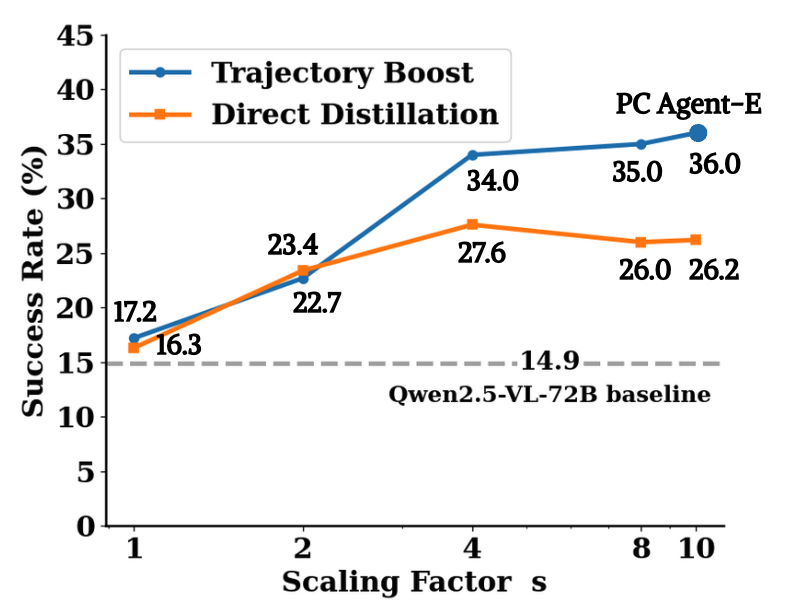
\includegraphics[width=0.6\linewidth]{assets/scaling.png}
    \caption{在 WindowsAgentArena-V2 上，Trajectory Boost 和直接蒸馏方法在不同数据扩展因子 $s$ 下的性能。}
    \label{fig:scale}
\end{figure}

\subsection{Trajectory Boost 与直接蒸馏的比较}
\label{subsec:distill_comparison}

为了说明我们的方法并非一种简单的蒸馏形式，我们将 Trajectory Boost 与直接蒸馏基线比较。对于该基线，我们直接从教师模型 Claude 3.7 Sonnet 端到端采样轨迹。我们还比较了将人类演示与直接蒸馏相结合的变体基线，详情见原文附录 D。

\paragraph{更优的性能。}
如图~\ref{fig:scale} 所示，在大多数训练数据规模下，我们的方法都显著优于直接蒸馏基线（蓝线对橙线）。作者将这一结果归因于合成数据的高质量。我们的方法以人类轨迹为可靠基础，利用前沿模型执行单步增强，从而避免端到端轨迹蒸馏中可能发生的误差累积。

\paragraph{出色的效率。}
本文方法的另一项显著优势是时间效率。蒸馏基线需要在虚拟机中部署 Claude，并通过在线交互收集轨迹，因此需要大量资源且十分耗时。相比之下，Trajectory Boost 无须与真实环境交互即可离线合成数据，并且天然易于并行。具体而言，在相同硬件条件下，为收集等量数据（3,120 条轨迹），蒸馏基线约需 \textbf{900 小时}，而 Trajectory Boost 只需 \textbf{3 小时}，实现了大幅的 \textbf{300 倍加速}。

\subsection{测试时扩展}
\label{subsec:test_time_scaling}

\begin{figure}[t]
    \centering
    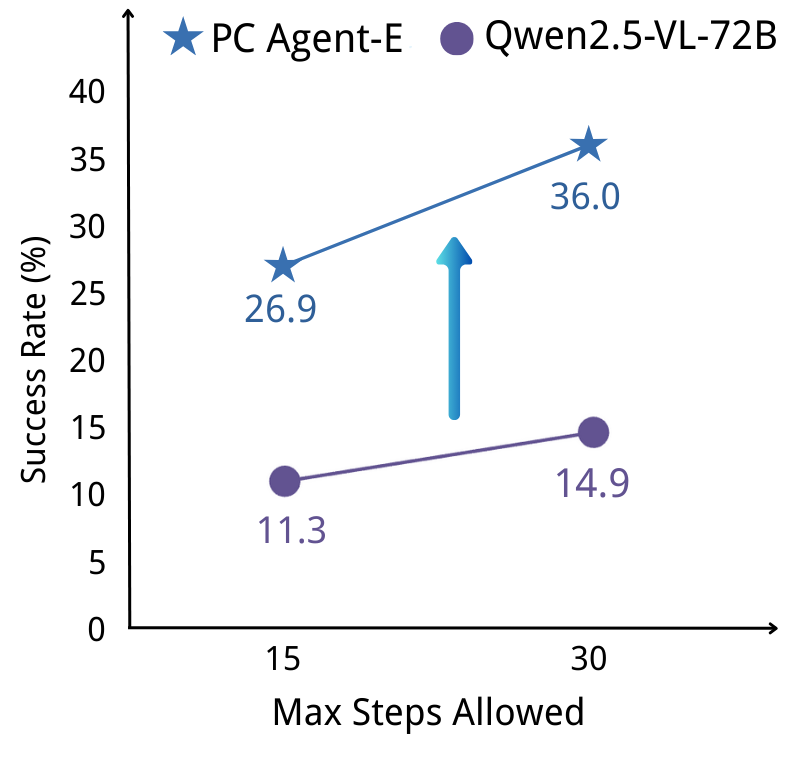
\includegraphics[width=0.46\linewidth]{assets/tts.png}
    \caption{WindowsAgentArena-V2 上的测试时扩展。}
    \label{fig:tts}
\end{figure}

我们还研究了 PC Agent-E 的性能如何随测试时扩展变化；这一主题正受到研究界越来越多的关注~\cite{wu2025inferencescalinglawsempirical,snell2024scalingllmtesttimecompute}。我们在完成任务时允许不同的最大步数，并评估模型性能。如图~\ref{fig:tts} 所示，当步数上限从 15 增至 30 时，PC Agent-E 能有效利用额外计算；允许的步数越多，它相对基础模型的性能差距就越大。这说明训练所获得的更强\textit{规划}能力，使 PC Agent-E 能够受益于更长的交互时域。原文附录 E 进一步将评估扩展到 50 步上限；作者在该设置下观察到轻微的性能下降，并分析了潜在原因。

\subsection{跨平台评估}
\label{subsec: osworld}

为了评估跨平台泛化能力，我们还在 OSWorld 上评估了模型。如表~\ref{tab:osworld} 所示，尽管 PC Agent-E 只在 Windows 数据上训练，它在 Linux 系统中也取得了 34\% 的相对提升。这些结果验证了本文方法的泛化能力。

\begin{table}[t]
  \centering
  \begin{tabular}{lccc}
    \toprule
    \textbf{模型} & \textbf{可行} & \textbf{不可行} & \textbf{总计} \\
    \midrule
    任务数 & 339 & 30 & 369 \\
    \midrule
    Qwen2.5-VL-72B & 4.4 & \textbf{86.7} & 11.1 \\
    \textbf{PC Agent-E（本文）} & \textbf{10.9} & 63.3 & \textbf{14.9} \\
    \bottomrule
  \end{tabular}
  \caption{OSWorld 上的成功率（\%，30 步）。}
  \label{tab:osworld}
\end{table}

我们还在该实验中发现一个有趣现象，即\autoref{sec:waa-v2} 所称的\textit{不可行任务投机}：较弱的 Qwen2.5-VL-72B 模型反而在不可行任务上取得了明显更好的表现。这一观察说明，当前针对不可行任务的评估无法准确反映计算机使用智能体的能力。未来研究可以为不可行任务设计更好的评判标准，例如在智能体声明任务不可能完成时检查其理由。

\section{结论}

本文提出 PC Agent-E，一种面向计算机使用智能体的高效训练框架。该框架采用 Trajectory Boost，这是一种利用前沿模型生成的多样化动作备选项增强人类演示的数据合成方法。PC Agent-E 仅使用 312 条增强轨迹进行训练，便相较基础模型取得了 141\% 的相对提升，甚至超过强教师模型 Claude 3.7 Sonnet。消融研究进一步表明，该方法不仅显著优于只使用人类轨迹，也比直接蒸馏教师模型更加高效、更加有效。这些发现说明，只需一小组高质量轨迹，就能有效激发复杂的计算机使用能力。

\section*{致谢}

我们衷心感谢 Shijie Xia 的细致审阅和建设性建议，这些意见显著提升了本文质量。本项目得到上海交通大学电子信息与电气工程学院（SJTU SEIEE）- 字节跳动大语言模型联合实验室及 SII 的支持。

\bibliography{main}
\bibliographystyle{main}

\end{document}
